\section{Introducción} \label{introduccion}



Para este trabajo nos centraremos en resolver un problema real de aprendizaje automático utilizando el conocimiento obtenido a lo largo de las asignaturas del máster, comenzando con un análisis exploratorio de datos, aplicación de técnicas de preprocesamiento, uso de técnicas de sobremuestreo, así como el desarrollo del modelo que aprenderá el sistema basado en reglas y el motor de inferencia.

\subsection{Problema a resolver}

De cara a la identificación de cadáveres, una de las tareas clave es la estimación de la edad. Aunque los forenses tenían formas de estimar a que edad murió una persona a partir de sus restos óseos, no existía un método concreto y universal de forma que el forense solo tuviera que seguir ciertas pautas y observar ciertas características para estimar la edad de un fallecido.

Por este motivo, en el año 1920, Thomas Wingate Todd publicó un artículo científico \cite{todd} en el que proponía una forma de clasificar en diez rangos de edad los restos óseos de una persona fallecida a partir de ciertas características de la sínfisis púbica, de forma que el proceso de identificación de cadáveres fuera más sencillo para los forenses.

A pesar de ser una publicación de hace más de cien años, este método sigue siendo la base para la estimación de la edad a partir de los restos óseos. La mayoría de técnicas actuales se basan en esta propuesta y se siguen aplicando de forma manual.

El sistema propuesto por Todd se centraba en nueve características, asignándole distintos valores categóricos, de la sínfisis púbica para realizar su clasificación:

\begin{enumerate}
	\item Crestas y surcos: Porosidad regular, muy definidas, poco profundas, crestas en formación, restos de surcos o no hay surcos.
	\item Superficie porosa irregular: No, medianamente o sí.
	\item Borde superior: Definido o no definido.
	\item Nódulo óseo: Ausente o presente.
	\item Borde inferior: Definido o no definido.
	\item Borde dorsal: Definido o no definido.
	\item Plataforma dorsal: Ausente o presente.
	\item Bisel ventral: Ausente, en proceso de formación o formado.
	\item Borde ventral: Ausente, parcialmente formado, formado sin excrecencias, formado con pocas excrecencias o formado con muchas excrecencias.
\end{enumerate}

\begin{table}[H]
\resizebox{\textwidth}{!}{%
	\begin{tabular}{|c|c|c|}
	\hline
	Crestas y surcos: Muy definidos & Superficie porosa irregular: Sí & Borde superior: Definido  \\ \hline
	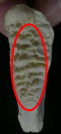
\includegraphics[scale = 0.75]{huesos/crestas_surcos_muy_definidos.png}  &   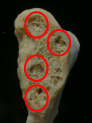
\includegraphics[scale = 0.75]{huesos/superficie_porosa_si.png} &  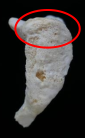
\includegraphics[scale = 0.75]{huesos/borde_superior_definido.png}  \\ \hline
	Nódulo óseo: Presente & Borde inferior: No definido & Borde dorsal: Definido \\ \hline
	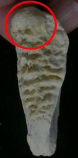
\includegraphics[scale = 0.75]{huesos/nodulo_oseo_presente.png} & 
\includegraphics[scale = 0.75]{huesos/borde_inferior_no_definido.png} &  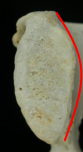
\includegraphics[scale = 0.75]{huesos/borde_dorsal_definido.png} \\ \hline
	Plataforma dorsal: Presente & Bisel ventral: En proceso de formación & Borde ventral: Muchas excrecencias \\ \hline
	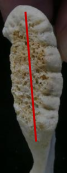
\includegraphics[scale = 0.75]{huesos/plataforma_dorsal_presente.png} & 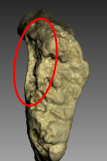
\includegraphics[scale = 0.75]{huesos/bisel_ventral_en_proceso_formacion.png} &   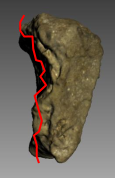
\includegraphics[scale = 0.75]{huesos/borde_ventral_muchas_excrecencias.png} \\ \hline
	\end{tabular}%
}
	\caption{Algunos ejemplos de las características consideradas por Todd.}\label{table:caracteristicas_todd}
\end{table}

Observando estas características Todd proponía una clasificación en diez fases:

\begin{itemize}
	\item Fase 1: 19 años.
	\item Fase 2: De 20 a 21 años.
	\item Fase 3: De 22 a 24 años.
	\item Fase 4: De 25 a 26 años.
	\item Fase 5: De 27 a 30 años.
	\item Fase 6: De 31 a 34 años.
	\item Fase 7: De 35 a 39 años.
	\item Fase 8: De 40 a 44 años.
	\item Fase 9: De 45 a 49 años.
	\item Fase 10: Más de 50 años.
\end{itemize}

Como era de esperar, podemos ver que las fases de edad más tempranas son más fáciles de asignar y los rangos de edad son más pequeños, mientras que en las fases más avanzadas los rangos de edad son mucho mayores, llegando a la última fase de más de 50 años, que aunque hoy en día nos parezca que gran parte de la población se asignaría a esa fase, en la época que Todd propuso esta clasificación la esperanza de vida era mucho menor.

En este problema se trata de un problema de clasificación ordinal, difícil de resolver debido a la complejidad en el conjunto de datos, además de requerir un modelo explicable de cara a ayudar a los expertos.

\subsubsection{Conjunto de datos}

Uno de los principales inconvenientes de este problema es que, como podemos ver, tenemos un gran número de características, de posibles valores para dichas características y de clases que asignar a cada dato, por lo que tendremos que buscar formas de tratar con la alta dimensionalidad del problema.

Por otro lado, es muy difícil obtener un buen conjunto de datos para este problema. En nuestro caso utilizaremos un conjunto de datos clasificado manualmente por el Laboratorio de Antropología Física de la Universidad de Granada\cite{laboratorioForenseUGR}.

Este conjunto está formado por datos tomados de ambas lateralidades de la sínfisis púbica, siendo en total 960 datos distribuidos en los diez rangos de edades propuestos por Todd.


\begin{figure}[H]
	\centering
	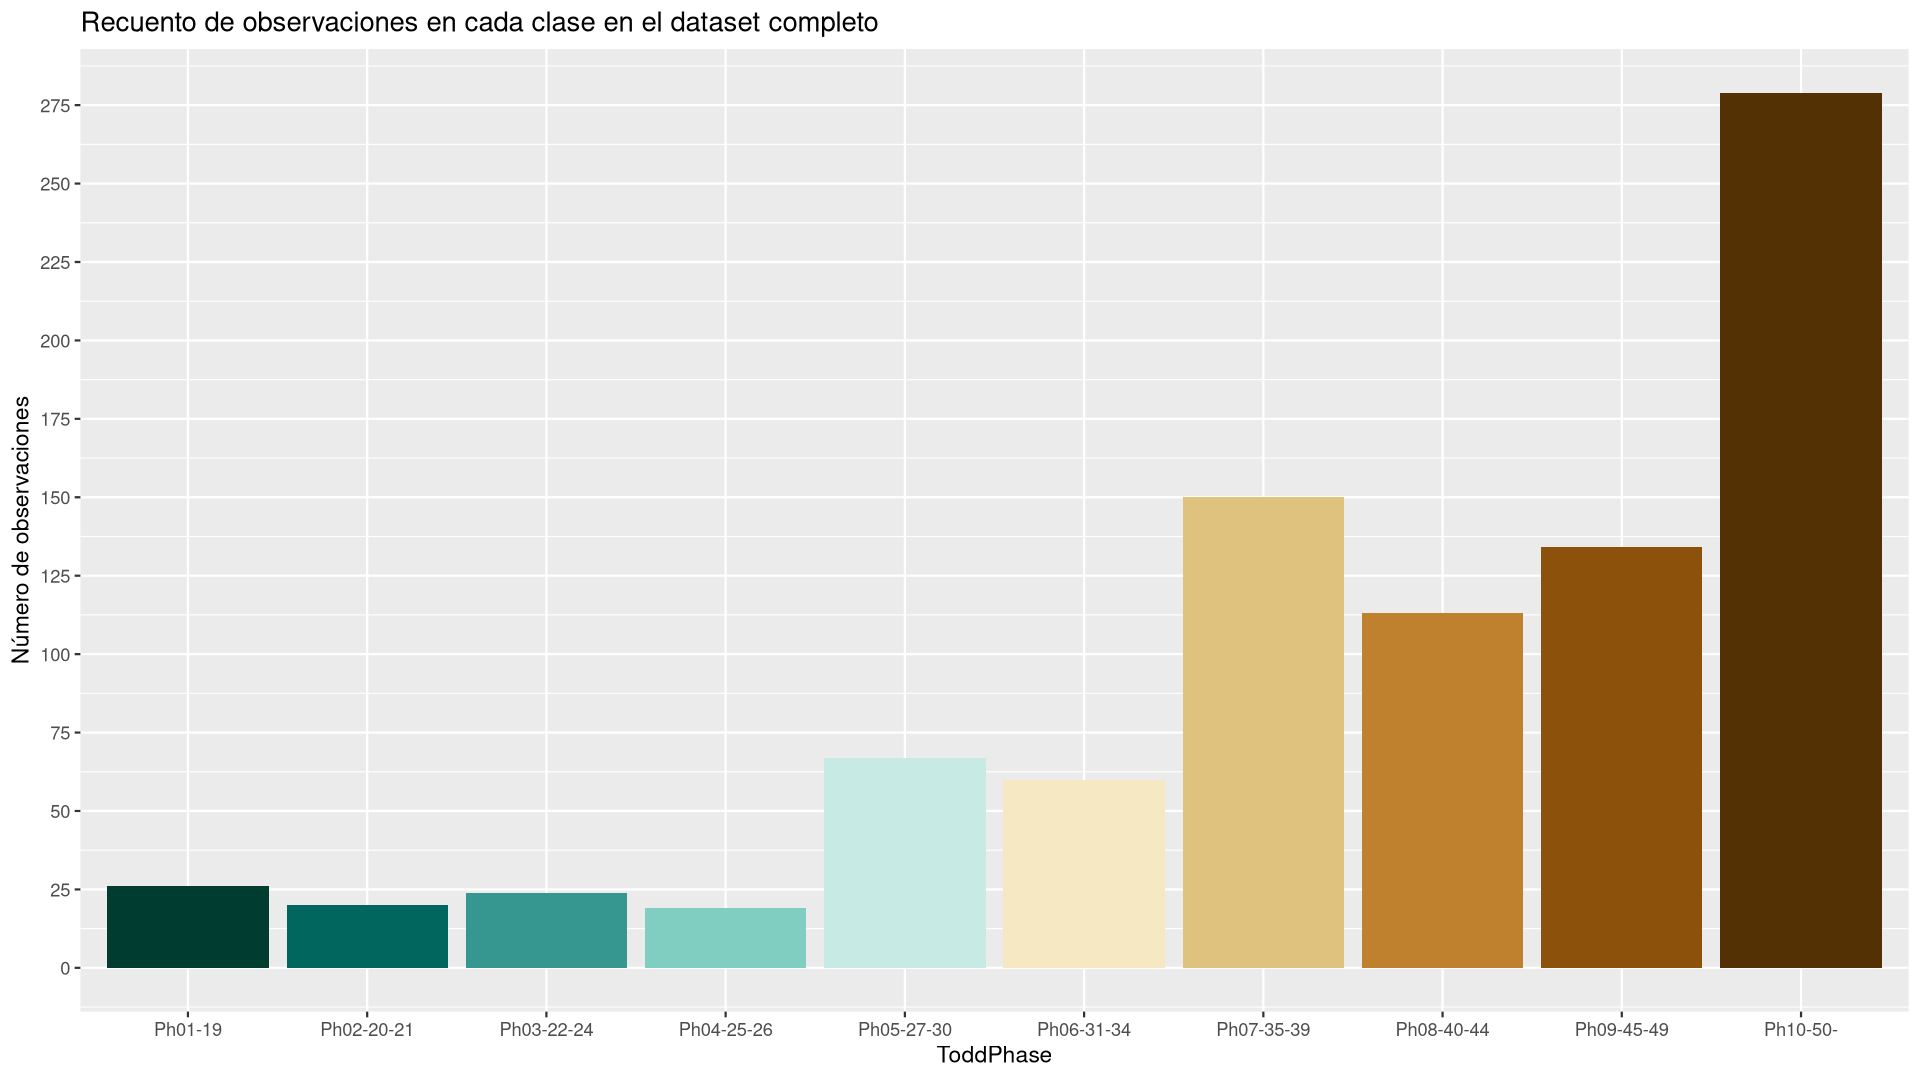
\includegraphics[width = \textwidth]{conjunto_datos/distribucion_clases_completo.png}
	\caption{Número de datos por cada fase propuesta por Todd con el conjunto de datos completo.}
	\label{fig:conteo_original}
\end{figure}


Como vemos, este conjunto de datos se encuentra claramente desbalanceado, hay muchas más muestras de las clases de edad más avanzada que de edades más bajas, además de contar con muy pocos en la mayoría de clases. Más adelante veremos como podemos solucionar estos problemas utilizando técnicas de sobremuestreo.

\subsection{Motivación}

Este trabajo está motivado porque la propuesta de Todd y sus trabajos derivados son demasiado subjetivos, haciendo muy poca distinción entre las fases y dejando gran parte del criterio de la estimación a cargo del forense.

Aunque en los últimos años se han desarrollado modelos de inteligencia artificial que son capaces de obtener buenos resultados en esta clase de problemas, los modelos actuales apenas son interpretables por los expertos y esto no les permite utilizarlos para avanzar en las técnicas de estimación de la edad a partir de restos óseos.

Por este motivo aparece la Inteligencia Artificial Explicable, y utilizando este tipo de técnicas intentaremos resolver el problema para que el experto sea capaz de entender y razonar como funciona el modelo.


\subsubsection{Inteligencia Artificial Explicable}

En la última década los distintos modelos de aprendizaje automático, como las redes neuronales, han revolucionado la inteligencia artificial. Estos nuevos modelos obtienen resultados impensables con modelos clásicos, aunque son demasiado complejos de interpretar. Por este motivo ha aparecido el concepto de Inteligencia Artificial Explicable \cite{XAI} (XAI de sus siglas en inglés).

La inteligencia artificial explicable trata de expresar modelos de inteligencia artificial de una forma simple e interpretable. Con esto se busca que no solo los desarrolladores de dichos modelos sean capaces de comprobar y validar como funciona el modelo, sino que los usuarios sean capaces de entender a grandes rasgos como funciona, ya que en muchas ocasiones han de ser capaces de interpretar las decisiones del modelo para realizar su trabajo.

En este trabajo, debido a la complejidad del problema, así como que el experto que utilizará los resultados del modelo ha de ser capaz de interpretar, validar, y tomar decisiones con los resultados del modelo, se buscará obtener un modelo simple y fácilmente interpretable. Por este motivo proponemos un sistema basado en reglas, donde se utilizará el algoritmo de Programación Genética para obtener el conjunto de reglas del sistema.

\newpage

\subsection{Objetivos}

Tras introducir el problema, comentar los principales retos que nos podemos encontrar y orientar que tipo de solución buscamos, podemos distinguir estos claros objetivos:

\begin{enumerate}
	\item Discutir la importancia de resolver este problema, así como los distintos enfoques utilizados hasta ahora en los distintos estudios que se han propuesto resolverlo.
	\item Estudiar y discutir distintos métodos de preprocesamiento de datos, en especial el balanceado de datos debido a las características del problema.
	\item Estudiar, desarrollar y entrenar algoritmos evolutivos que permitan inferir reglas a partir de un conjunto de datos, discutiendo y analizando las distintas técnicas utilizadas hasta el momento para esta tarea.
	\item Implementar un sistema basado en reglas capaz de resolver el problema.
	\item Estudiar la idoneidad de la solución propuesta para el problema teniendo en cuenta tanto su factor de acierto como su interpretabilidad de cara a ser usado por expertos en el problema.
\end{enumerate}


\newpage
